\chapter{SCADA}
\label{ch:scada}
%Finalmente y para resumir la evolución del proyecto hasta este punto
Para continuar en el desarrollo es necesario analizar los pasos antes descriptos 
para la construcción de la planta. De esta manera, en el capitulo 
\ref{ch:DisenoEnsamblado} detallamos el sistema físico de la misma, lo que nos 
condujo a describir en el capitulo \ref{ch:tablero} el sistema eléctrico y 
electrónico que la anima, continuamos en el capitulo \ref{ch:progPLC} con la 
lógica que regula al sistema completo por medio del \gls{plc}. 

Como elemento final de este \gls{pfe} se diseño y realizo una \gls{hmi} 
\gls{scada} mediante P-CIM para Windows de AFCON con el objetivo de poder 
manipular la planta/el sistema sin tener un acceso físico a la misma.

En el siguiente capítulo se detallan cada uno de los pasos seguidos para la 
realización de tal interfaz así como también la configuración actual. Mediante 
la información que se brinda en esta sección el lector podrá entender y por lo 
tanto modificar en caso de ser necesario todo el entorno \gls{scada}. Sin 
embargo, este capitulo no esta orientado a la operación misma de la planta 
mediante el \gls{scada} lo cual se detalla en la sección \todo{agregar la 
sección donde se describe la operación mediante el scada}

\section{Introducción a SCADA}
\label{sec:IntroScada}
Aunque un \gls{plc} realiza automáticamente un control pre-programado sobre un 
proceso, no tienen una manera estándar de presentar la información al operador y 
ademas suelen estar distribuidos a lo largo de toda la planta, haciendo difícil 
recoger los datos de manera manual.%para poder concentrarlos
En cambio, los sistemas \gls{scada} obtienen los datos de manera 
automática desde múltiples \gls{plc} o desde otros controladores por medio de 
algún tipo de red de extensión variable, facilitando la tarea de concentrar 
los datos. Se puede observar en la Fig.\ref{fig:perspectivaSCADA} la 
organización esquemática de un sistema Planta-PLC-SCADA.
\begin{figure}[ht!]
	\centering
	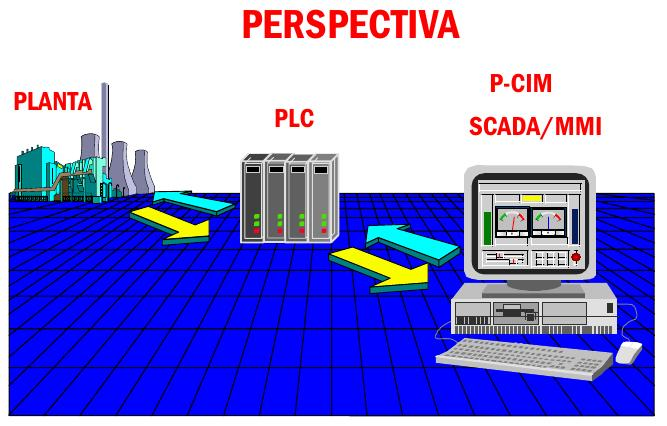
\includegraphics[width=0.445\textwidth]
	{Cap5-SCADA/images/perspectiva.jpeg}
	\caption{Diagrama de un sistema SCADA}
	\label{fig:perspectivaSCADA}
\end{figure}

Un sistema \gls{scada} recopila constantemente información de la planta en 
tiempo real. Luego mediante una base de datos se almacenan y evalúan los datos, 
generandose alarmas en los casos correspondientes. Finalmente, mediante 
la \gls{hmi} se brinda la información al operario y este a su vez puede enviar 
instrucciones a los \gls{plc} en la planta. También se pueden incluir datos de 
diagnóstico y manejo de la información así como un cronograma de procedimientos 
de mantenimiento, información logística, esquemas detallados para un sensor o 
máquina en particular o incluso sistemas expertos con guía de resolución de 
problemas. 

Es entonces claro que la utilización de un sistema \gls{scada} reduce 
fuertemente las tareas asociadas al control y monitoreo de plantas industriales.

\section{Scada P-CIM}
\label{sec:ScadaPCIM} 
Para el diseño y desarrollo del sistema \gls{scada} de este \gls{pfe} se 
utilizó el software P-CIM 7.70 SP4 para Windows de AFCON 
(\url{www.afcon-inc.com}). El mismo, provee de un ambiente tanto de desarrollo 
como de ejecución de aplicaciones \gls{scada}. Este software puede ser 
descargado desde la pagina de \href{
http://www.afcon-inc.com/Templates/showpage.asp?TMID=108&FID=733&PID=0&IID=8334}
{P-CIM 7.70 SP4}.

Dentro de las características que ofrece este sofware se encuentran:
\begin{itemize}
 \item Compatible con todas las plataformas MS-Windows actuales.
 \item Soporta un gran número de diferentes \gls{plc} y otros dispositivos 
  periféricos.
 \item Posee drivers para diversos buses de comunicación.
 \item Provee herramientas para el desarrollo de \gls{hmi} inteligentes 
 \item Permite el seguimiento de los procesos de la planta y las actividades de 
 los operadores
 \item Brinda un entorno para monitorear alarmas y eventos en toda la extensión 
 de la planta
\end{itemize}


\subsection{Estructura de P-CIM}
\label{sec:CapasPrograma}
P-CIM presenta una estructura que se divide en tres grandes capas de 
abstracción. Dicha estructura se puede observar en la 
Fig.\ref{fig:estructuraSCADA}, donde ademas se detallan los diferentes 
componente de P-CIM que intervienen en cada una de ellas.
\begin{figure}[ht!]
\centering
	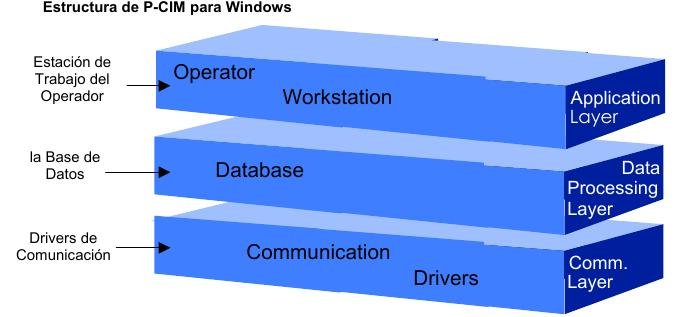
\includegraphics[width=0.5\textwidth]
	{Cap5-SCADA/images/estructura.jpeg}
	\caption{Esquema de la estructura en capas de P-CIM}
	\label{fig:estructuraSCADA}
\end{figure}

\begin{itemize}
 \item Capa de Comunicación: Se encarga de la comunicación entre el \gls{plc} y 
 la PC. Por ello es necesario la instalación y configuración de un driver que 
 gestione tal comunicación. Ver Sec.\ref{subsec:CapaComunicacion}.
 \item Capa de Procesamiento de Datos: Donde por medio de una base de datos se 
lleva a cabo el procesamiento de datos, registro histórico y manejo de alarmas. 
Ver Sec.\ref{subsec:CapaProcesamiento}.
 \item Capa de aplicación: Presenta la información, interactúa con el operador 
  y realiza los controles de alto nivel y de programación. Esta tarea 
\end{itemize}

El trabajo coordinado se resume en que la información de campo del PLC llega al 
\gls{scada} a través de la capa de comunicación. Esta se transfiere a la Capa de 
Procesamiento de Datos (Servidor de la Base de Datos o Database Server) donde se 
analiza. La capa de aplicación la procesa y envía hacia el Operator 
Workstation(\gls{hmi}). De esta manera el funcionamiento conjunto de cada una de 
estas capas permite al sistema \gls{scada} funcionar de manera correcta y con 
las prestaciones antes mencionadas.


\section{Desarrollo de la aplicacion SCADA con P-CIM}
A continuación, se detalla la aplicación \gls{scada} desarrollada para este 
\gls{pfe} en el software P-CIM. Su exposición esta dividida de acuerdo a la 
estructura en capas del programa, como se describió en la sección 
\ref{sec:CapasPrograma}.

\subsection{Capa de comunicación}
\label{subsec:CapaComunicacion}
El primer paso para el desarrollo de un sistema \gls{scada} es lograr la 
comunicación por medio de algún bus con el \gls{plc} que controla la planta. Es 
decir, lograr un buen funcionamiento de la capa de comunicación. En nuestro caso 
se utilizó el protocolo de comunicaciones Modbus. 

\subsubsection{Modbus}
Modbus es un protocolo de comunicaciones diseñado en 1979 por Modicon para su 
gama de \gls{plc}. En abril del 2004, Schneider Electric transfirió los 
derechos a la la Modbus Organization \url{http://www.modbus.org/}, la cual se 
encarga desde entonces del desarrollo y actualización del protocolo Modbus.

Para la conexión entre un computador corriendo un software \gls{scada} y uno o 
varios \gls{plc} el protocolo Modbus es un estándar de facto en la industria . 
Por esta razón, también, goza de una gran disponibilidad para la conexión de 
dispositivos electrónicos industriales. A nivel diseño, se encuentra situado en 
la capa de aplicación según el modelo \gls{osi} y presenta una arquitectura 
maestro/esclavo o cliente/servidor.

Las principales razones para el uso de Modbus:
\begin{itemize}
 \item Simple y robusto
 \item Fue desarrollado para aplicaciones industriales.
 \item Su implementación es fácil y requiere poco mantenimiento.
 \item Maneja bloques de datos sin suponer restricciones a los vendedores.
 \item Permite la comunicación entre múltiples dispositivos en la misma red. 
  Aprox. 240
 \item De código abierto y libre de regalías.%openly published and royalty-free
\end{itemize}


\subsubsection{Instalación Driver Modbus}
A continuación se detalla el  proceso de configuración y puesta en marcha del 
bus de comunicaciones. El driver de para Modbus se puede descargar desde esta 
\href{http://www.afcon-inc.com/afcon/Templates/showpage.asp?TMID=402&FID=832}{pagina}.
Para realizar la instalación de este driver de comunicaciones en P-CIM seguimos 
los siguientes pasos:(Ver Tab.\ref{tab:installModbus})
% \begin{enumerate}
%  \item Elija $Setup~de~P-CIM$ del grupo de aplicaciones que se encuentran la carpeta $AFCON~P-CIM[7.70SP4]$.
%  \item Aparecerá en la pantalla la ventana de $Setup~de~P-CIM$. Elija $Install~P-CIM~Driver$.
%  \item La ventana de diálogo de instalación del Driver de P-CIM, le pedirá que indique el directorio del driver.
%        Oprima Browse.
%  \item Seleccione el directorio de origen del driver para Modbus. En nuestro caso $C:/P-CIM32.BAK/DRIVERS/MODBUS.689$.
%  Oprima OK y luego Next.
%  \item El Setup de P-CIM despliega la ventana de diálogo de Bienvenida. Para continuar, oprima Next. 
%  \item El Setup de P-CIM despliega la ventana de diálogo de Propiedades del Driver de P-CIM 
%   para Windows 32, indicando los detalles del driver a ser instalado.
%  \item Elija el/los proyecto(s) en los que Ud. desea instalar el driver o bien seleccione
%   All (todos) y oprima Next.
%   \item El Setup de P-CIM procede a efectuar la instalación y finalmente muestra este mensaje: 
%   “La instalación del driver se ha completado”. Oprima OK para que desaparezca el cuadro de diálogo.
% \end{enumerate}
\begin{table}[H]
\small
\centering
\renewcommand*{\arraystretch}{0.3}
\begin{tabular}{*{2}{m{0.435\textwidth}}}
\hline
  Elija Setup de P-CIM del grupo de aplicaciones que se encuentran la carpeta 
  AFCON P-CIM[7.70SP4]. 
  &\begin{center}
    %\rule{0.4\textwidth}{0.3\textwidth}
    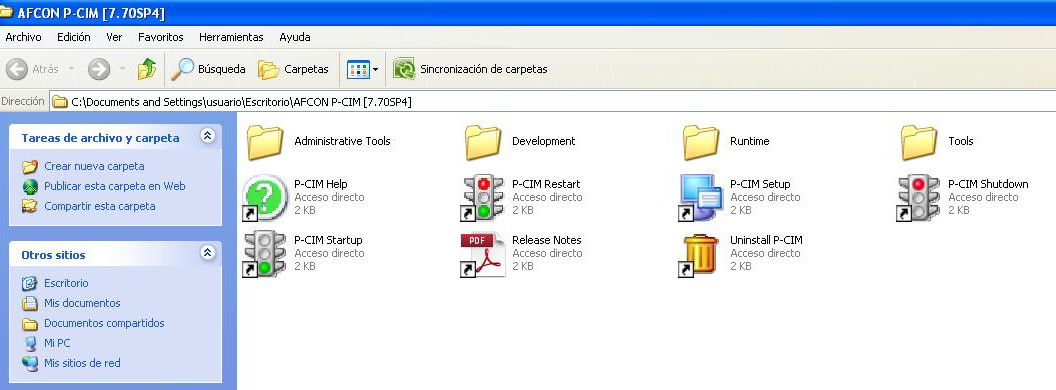
\includegraphics[width=0.4\textwidth]
	{Cap5-SCADA/images/Dibujo1.JPG}
  \end{center}\\
\hline
  De la ventana de Setup de P-CIM seleccione Install P-CIM Driver.
  Se desplegará la ventana de diálogo de instalación del Driver de P-CIM;
  &\begin{center}
    %\rule{0.4\textwidth}{0.3\textwidth}
    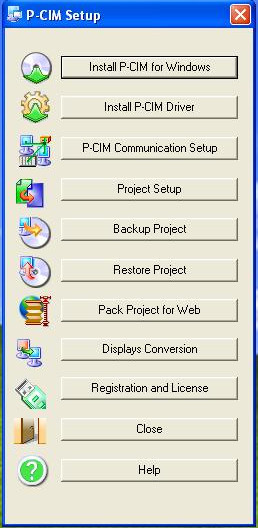
\includegraphics[height=0.3\textwidth]
	{Cap5-SCADA/images/PcimSetup.jpeg}
  \end{center}\\
\hline
  La ventana Install P-CIM driver le pedirá que indique el directorio del
  driver. Seleccione el directorio de origen del driver para Modbus. En este
 proyecto \texttt{C:\slash P-CIM32.BAK\slash DRIVERS\slash MODBUS.689}.
 Oprima OK y luego Next.
  &\begin{center}
    %\rule{0.4\textwidth}{0.3\textwidth}
    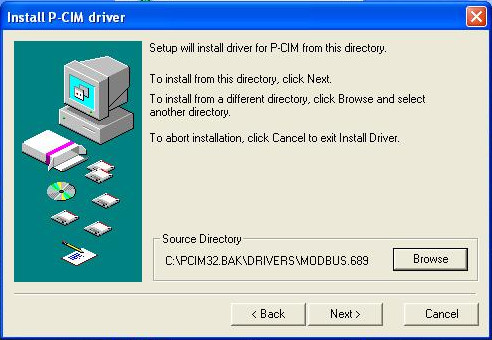
\includegraphics[width=0.4\textwidth]
    {Cap5-SCADA/images/installDriver.jpeg}
  \end{center}\\
\hline
 Se despliega la ventana de diálogo de Bienvenida, oprima Next. 
 Aparecerá la ventana de diálogo de Propiedades del Driver de 
 P-CIM, indicando los detalles del driver a ser instalado.
 Elija el/los proyecto(s) en los que Ud. desea instalar el driver o bien 
 seleccione All (todos) y oprima Next.
 Se efectuará la instalación y finalmente se muestra el mensaje “La instalación 
 del driver se ha completado”. Oprima OK para que desaparezca el cuadro de 
 diálogo.
  &\begin{center}
    %\rule{0.4\textwidth}{0.3\textwidth}
    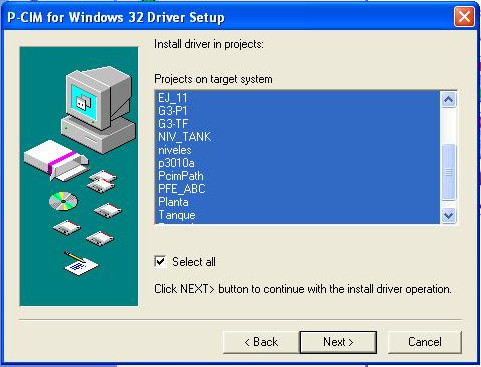
\includegraphics[width=0.4\textwidth]
    {Cap5-SCADA/images/installDriver2.jpeg}
  \end{center}\\
\hline
\end{tabular}
\caption{Instalación del Driver Modbus}
\label{tab:installModbus}
\end{table}

\subsubsection{Configuración Driver Modbus}
Una ves que el driver de Modbus para PCIM se ha instalado correctamente 
procedemos a realizar su configuración para lograr la comunicación entre el PLC 
y la computadora de control. Esta tarea se divide en dos partes: 
\begin{itemize}
 \item Asociar el driver con un puerto P-CIM:(Ver Tab.\ref{tab:ConfigModbus})\\
  P-CIM soporta 255 puertos lógicos, nombrados de 1 al 255.
%  \begin{enumerate}
%   \item Elija el Setup de P-CIM del grupo P-CIM para Windows 32.
%   \item  Elija el Setup de Comunicación de P-CIM (ALT+M). El Setup de P-CIM
%   despliega la ventana de diálogo “Project Communication Setup” de P-CIM.
%   \item Para agregar una nueva asociación driver-puerto, elija New.
%   \item Para editar una asociación existente, marque la línea correspondiente y
%   elija Edit.
%   \item El Setup de P-CIM despliega la ventana de diálogo “Port properties” 
%   (propiedades de puerto).
%   \item Ingrese el número de puerto entre 1 y 255 en la lista de Nombres de 
%   Puerto de la ventana.
%   \item Elija el nombre del driver de la lista de Driver Name (la lista 
% contiene nombres de drivers instalados en el proyecto en curso).
%   \item En el cuadro elija la notación numérica del bit – octal, decimal o 
%    hexadecimal – de la lista de Bit numbering system.
%   \item Elija la notación usada para referenciar el bit menos significativo – 0 
%    ó 1 – de la lista de Lowest bit number (Numeración del Menor Bit).
%   \item Para utilizar el driver en modo emulador, selecciones la casilla de 
%   Emulación.
%  \end{enumerate}
  \begin{table}[!ht]
  \centering
  \renewcommand*{\arraystretch}{0.3}
  \begin{tabular}{*{2}{m{0.435\textwidth}}}
  \hline
    Elija el Setup de P-CIM del grupo P-CIM para Windows 32.
    Elija el Setup de Comunicación de P-CIM, de donde se despliega la ventana 
    de diálogo "Project Communication Setup" de P-CIM.
    &\begin{center}
      %\rule{0.4\textwidth}{0.3\textwidth}
      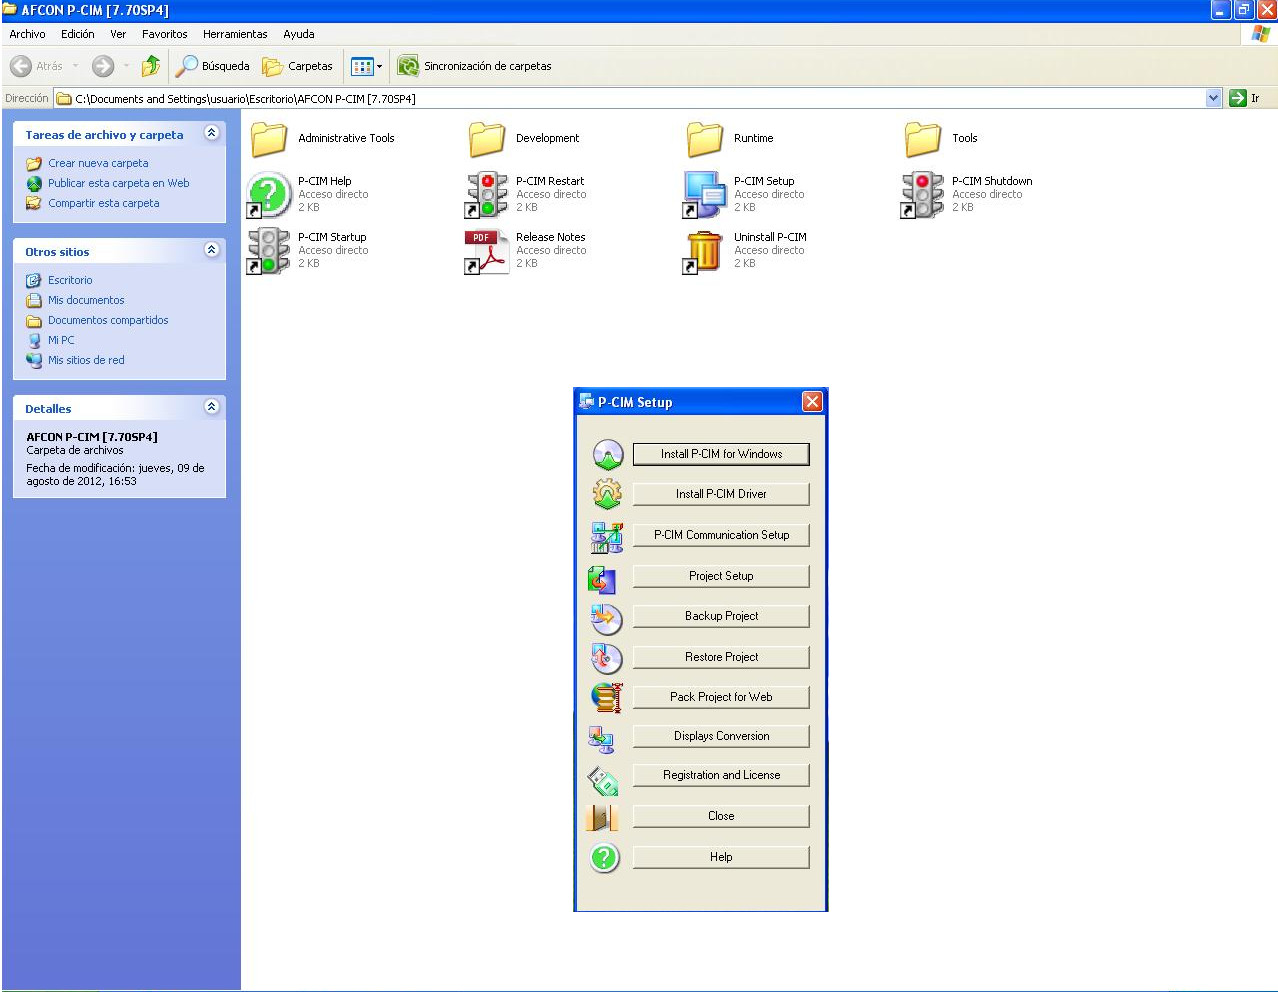
\includegraphics[width=0.4\textwidth]
	{Cap5-SCADA/images/SetupPCIM.JPG}
    \end{center}\\
  \hline
    Para agregar una nueva asociación driver-puerto, elija New.
    Para editar una asociación existente, marque la línea correspondiente
    y elija Edit
    &\begin{center}
      %\rule{0.4\textwidth}{0.3\textwidth}
       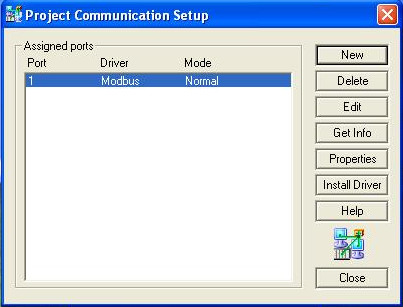
\includegraphics[width=0.4\textwidth]
	{Cap5-SCADA/images/commSetup.jpeg}
    \end{center}\\
  \hline
    Ingrese el número de puerto entre 1 y 255 en la lista de Nombres de 
    Puerto de la ventana.
    Elija el nombre del driver de la lista de Driver Name (la lista 
    contiene nombres de drivers instalados en el proyecto en curso).
    En el cuadro elija la notación numérica del bit – octal, decimal o 
    hexadecimal – de la lista de Bit numbering system.
    Elija la notación usada para referenciar el bit menos significativo –0 
    ó 1 – de la lista de Lowest bit number (Numeración del Menor Bit).
    Para utilizar el driver en modo emulador, selecciones la casilla de 
    Emulación.
    &\begin{center}
      %\rule{0.4\textwidth}{0.3\textwidth}
       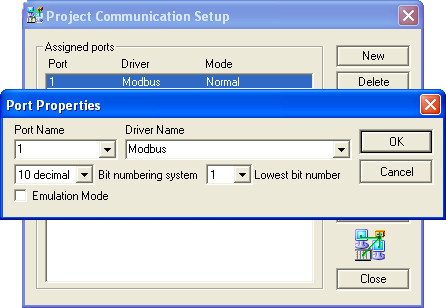
\includegraphics[width=0.4\textwidth]
	{Cap5-SCADA/images/portProp.jpeg}
    \end{center}\\
  \hline
  \end{tabular}
  \caption{Configuracion del Driver Modbus}
  \label{tab:ConfigModbus}
  \end{table}
 
  \item Establecer los parámetros operativos del puerto:(Ver 
    Tab.\ref{tab:PropModbus}\\
    En esta etapa Ud. define las propiedades de un driver para cada 
    puerto(lógico) de P-CIM con el que está asociado.
%  \begin{enumerate}
%   \item Elegir el Setup de P-CIM del grupo P-CIM para Windows 32.
%   \item Elegir el Setup de Comunicación de P-CIM (ALT+M). El Setup de P-CIM
%   despliega la ventana de diálogo Project Communication Setup.
%   \item Marque la línea correspondiente en el cuadro de Puertos Asignados y elija
%   Properties.
%   \item El Setup de P-CIM despliega la ventana de diálogo driver específico. 
%   Para el caso de Modbus se despliega la ventana P-CIM Configurator for MODBUS 
%   Driver
%   \item Elija el numero del puerto de P-CIM de la lista P-CIM Port
%   \item Defina la tabla de Polling mediante el botón Polling Configuration
%   \item Establezca el tipo de interfaz mediante la lista de Network Type en 
%   RS232. 
%   \item Transport Parameter despliega una ventana en la que se debe configurar 
% el puerto serial con  el mismo nombre con el que aparece en el Administrador de 
% Dispositivos de Windows.
%  \end{enumerate} 
\end{itemize}
\begin{table}[!ht]
\centering
\renewcommand*{\arraystretch}{0.01}
\begin{tabular}{*{2}{m{0.45\textwidth}}}
\hline
  Nuevamente desde la ventana de diálogo “Project Communication Setup” de 
  P-CIM marque la línea correspondiente en el cuadro de Puertos Asignados y 
  elija  Properties. El Setup de P-CIM despliega la ventana de diálogo driver 
  específico. Para el caso de Modbus se despliega la ventana P-CIM Configurator 
  for MODBUS Driver. Elija el numero del puerto de P-CIM de la lista P-CIM Port.
  &\begin{center}
    %\rule{0.4\textwidth}{0.3\textwidth}
    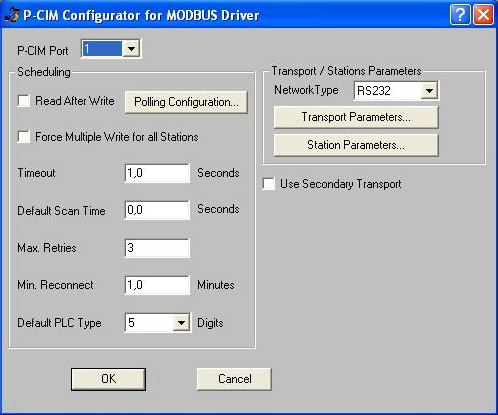
\includegraphics[width=0.4\textwidth]
      {Cap5-SCADA/images/modbusDriver.jpeg}
  \end{center}\\
\hline
  Defina la tabla de Polling mediante el botón Polling Configuration. En esta 
  se debe definir Start Address en 40001 segun se explica en la 
  Sec.\ref{subsubsec:InforDriver}.
  &\begin{center}
    %\rule{0.4\textwidth}{0.3\textwidth}
        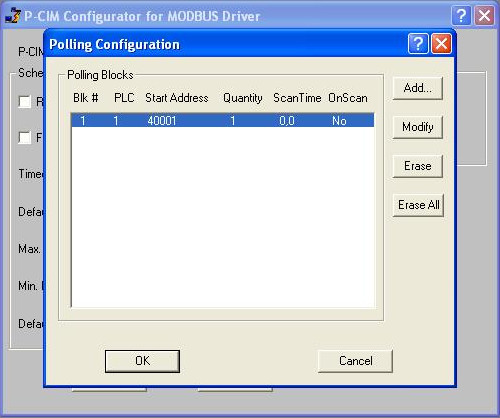
\includegraphics[width=0.4\textwidth]
      {Cap5-SCADA/images/modbusDriver1.jpeg}
  \end{center}\\
\hline 
   Establezca el tipo de interfaz mediante la lista de Network Type en RS232. 
   El botón Transport Parameter despliega una ventana en la que se debe 
   configurar el puerto serial con  el 
   mismo nombre con el que aparece en el Administrador de Dispositivos de 
   Windows.
  &\begin{center}
    %\rule{0.4\textwidth}{0.3\textwidth}
        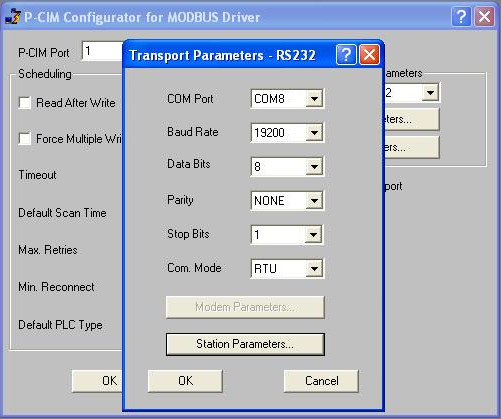
\includegraphics[width=0.4\textwidth]
      {Cap5-SCADA/images/modbusDriver2.jpeg}
  \end{center}\\
\hline
\end{tabular}
\caption{Propiedades del Driver Modbus}
\label{tab:PropModbus}
\end{table}

\subsubsection{Direccionando Información del Driver}
\label{subsubsec:InforDriver}
El acceso directo es el método por el cual los programas de aplicación (por
ejemplo, la base de datos) recuperan la información recibida directamente de 
los drivers de comunicación.

El formato en el cual las direcciones externas son especificadas en las
aplicaciones de P-CIM (Database, Animation Editor, y Operator
Workstation) es driver-dependiente. Estas son referenciadas especificando:
\begin{itemize}
 \item Server:El nombre del servidor es DBSR
 \item Topic: El nombre del tópico es PCIM
 \item Item: Especificado en el formato genérico Port:PLC:Address:Bit, en
  el que:
  \begin{itemize}
   \item Port number: el puerto de P-CIM asignado utilizado para la 
    información, 
    tal como se especificó en el Setup de Comunicación de P-CIM.
   \item PLC number: el número del PLC en la red de PLC (la sintaxis es driver-
    dependiente).
    \item Address: la dirección del dato o registro. La sintáxis depende 
    directamente del driver. Siendo para el driver Modbus la direccion 40001 el 
    equivalente directo a MW0 en el \gls{plc}
    \item Bit number: (opcional) el número de un bit específico en una palabra 
    o registro.
  \end{itemize}
  Ejemplo: 1:1:40001:2 hace referencia al bit 2 del registro 40001 o MW0 en el 
  PLC 1 que está conectado al Puerto 1.
\end{itemize}

\subsubsection{Verificación comunicación}
En este punto podemos verificar que la comunicación entre el PLC y la
computadora de control se haya establecido. Para monitorear el estado 
de la comunicación podemos utilizar las siguientes herramientas:
\begin{itemize}
 \item Sumario de Alarmas(Alarm Summary):\\
  Despliega mensajes del Sistema de Arranque, uno de los cuales es: “MODBUS
  Driver successfully loaded” indicando que el driver halló la tabla de 
  comunicación y fue exitosamente cargado.Ver Fig.\ref{fig:alarmsummary}
  \begin{figure}[!ht]
	\centering
	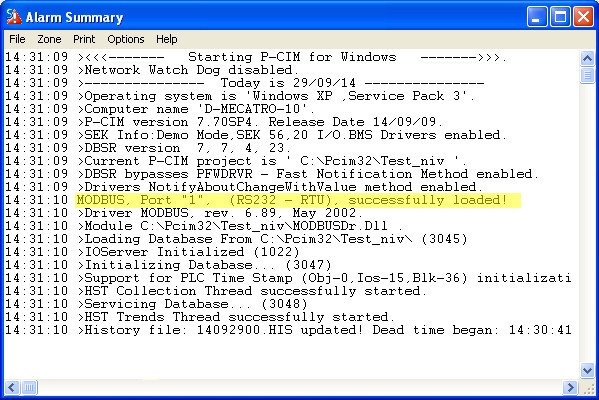
\includegraphics[width=0.8\textwidth]
	{Cap5-SCADA/images/alarm.jpeg}
	\caption{Ventana Alarm Summary con conexión Modbus Exitosa}
	\label{fig:alarmsummary}
  \end{figure}
 \item Monitor de Datos (Datascope):\\
  Esta herramienta se encuentra dentro del subdirectorio Tools.
  Para verificar el estado de la comunicación,
  debe ingresar en el Monitor de Datos cualquier dirección de PLC que esté 
  definida en la tabla de Polling. Al hacerlo, Ud. tendrá un valor por la 
  dirección que insertó,
  indicando que la comunicación está funcionando, o bien recibirá un cero, y
  después de un momento se desplegará un mensaje en la ventana de Resumen
  de Alarma, indicando que la comunicación falló. Véase la 
  sección\ref{subsubsec:InforDriver} para mas información acerca de las 
  direcciones del PLC y la base de datos. Ver 
  Fig.\ref{fig:dataScope}
  \begin{figure}[!ht]
	\centering
	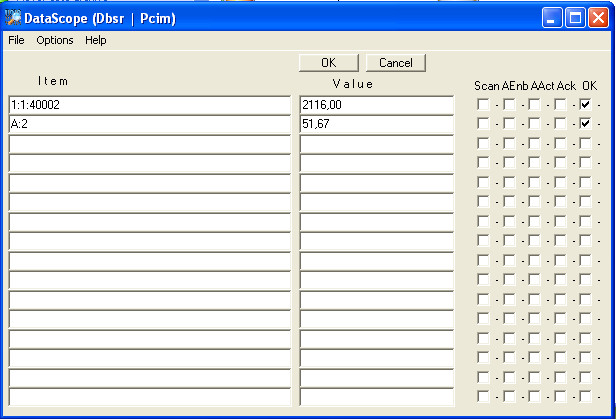
\includegraphics[width=0.4\textwidth]
	{Cap5-SCADA/images/dataScope.jpeg}
	\caption{Ventana de DataScope}
	\label{fig:dataScope}
  \end{figure}
\end{itemize}


\subsection{Capa de procesamiento}
\label{subsec:CapaProcesamiento}
Una ves que hemos verificado que se ha establecido la comunicación con el 
\gls{plc}, nos ocuparemos de la base de datos de P-CIM. Esta se encarga de 
recuperar, almacenar y procesar la información de tiempo real e histórica de los 
controladores, dispositivos periféricos y variables internas. Es decir, la base 
de datos conforma la capa de procesamiento.

La base de datos esta formada por elementos llamados bloques que son utilizados 
para:
\begin{itemize}
 \item Proporcionar una interfaz con el operador.
 \item Generar alarmas.
 \item Intercambiar información.
 \item Registrar información a ser usada en las tendencias.
 \item Convertir información en unidades de ingeniería.
\end{itemize}
La creación de los bloques de la base de datos es un paso importante que 
debe ser llevado a cabo después de establecer las comunicaciones.

\subsubsection{Diseño de la base de datos}
Para configurar y editar la base de datos se utiliza el programa 
Editor de la Base de Datos que se encuentra dentro del sub-directorio 
Development. Al crear la base de datos, se deben tener en cuenta los 
siguientes puntos:
\begin{itemize}
  \item Tipo de Bloque:\\Existen 8 tipos de bloques de base de datos para el
    manejo de 4 tipos básicos de datos: analógicos (enteros o reales),digitales 
    (un solo bit), string o cadena de caracteres (veinte palabras de 16 bits) y
    alarmas (en grupos de 16 bits)
  \item Tiempo de Escrutinio (scan) y de Fase:\\Que son respectivamente:
    \begin{itemize}
      \item El intervalo entre sucesivos procesamientos del bloque.
      \item El tiempo inicial de demora entre la carga de la base de datos 
      hasta el primer procesamiento del bloque.
    \end{itemize}
    Ambos en el orden de 1-255 unidades donde la unidad de tiempo por defecto es 
    un segundo.
  \item Alarmas:\\Las alarmas pueden ser definidas para los bloques de Valor 
    Analógico, Valor Digital, de Cálculo y Booleanos.
  \item Tendencias en tiempo real a corto plazo (S.T.) e Histórica (H.T.):\\son 
    el número de lecturas (0-255) a ser promediadas para cada punto 
    \begin{itemize}
      \item en un gráfico de tendencia en tiempo real.
      \item registrado en el archivo de tendencia histórica
    \end{itemize}
    respectivamente.
  \item Target y Targetlogic:\\Los bloques del target son campos de la base de 
    datos que reciben valores de otros bloques de la base de datos.
  \item Aseguramiento (Clamping):\\Es utilizado para limitar la salida de un 
    bloque de la base de datos o la entrada de un control a una especificada 
    amplitud de valores superior/inferior.
  \item Inversión:\\ Invierte los valores de la entrada desde el dispositivo y 
    los valores de la salida hacia el dispositivo.
\end{itemize}

Ahora, teniendo en cuenta las variables establecidas en el \gls{plc} 
para la comunicación con el \gls{scada} (Ver 
tablas \ref{table:bitlecturasescrituras} y 
\ref{table:palabraslecturasescrituras}) podemos definir los bloques de la base 
de datos que serán necesarios. Estos bloques los dividimos en tres 
grandes grupos con configuraciones similares:
 
\begin{itemize}
 \item Analog Input/Output: Bloque analógico con información desde/hacia el 
  \gls{plc} a la base de datos. Debemos definir entradas a la base de datos con 
  la dirección del espacio de memoria en el \gls{plc} para poder acceder en 
  Lectura/Escritura en estos registros.
 \item Calculation:  Conversiones en unidades de ingeniería o porcentual 
  según sea necesario. Las variables leídas del \gls{plc} estan definidas en 
  una escala de $0$ a $4095$ por esta razón deben ser convertidas para
adaptarse tanto al \gls{plc} como al \gls{hmi} del \gls{scada}.
 \item Analog Emulation: Bloque analógico con información hacia/desde el 
  \gls{hmi} del \gls{scada} a la base de datos. Es necesario definir variables 
  internas del \gls{scada} para ser utilizadas para lectura/escritura de la 
  \gls{hmi}.
\end{itemize}

En la figura \ref{fig:bloqDB} se presenta un esquema que sintetiza la 
configuracion de los bloques que forman la base de datos. En esta, se observa 
como el dato que se origina del lado \gls{plc} o \gls{hmi} viaja hasta el otro 
lado por medio de la base de datos.

\begin{figure*}[!ht]
  \centering 
  \resizebox{\textwidth}{!}{
  
  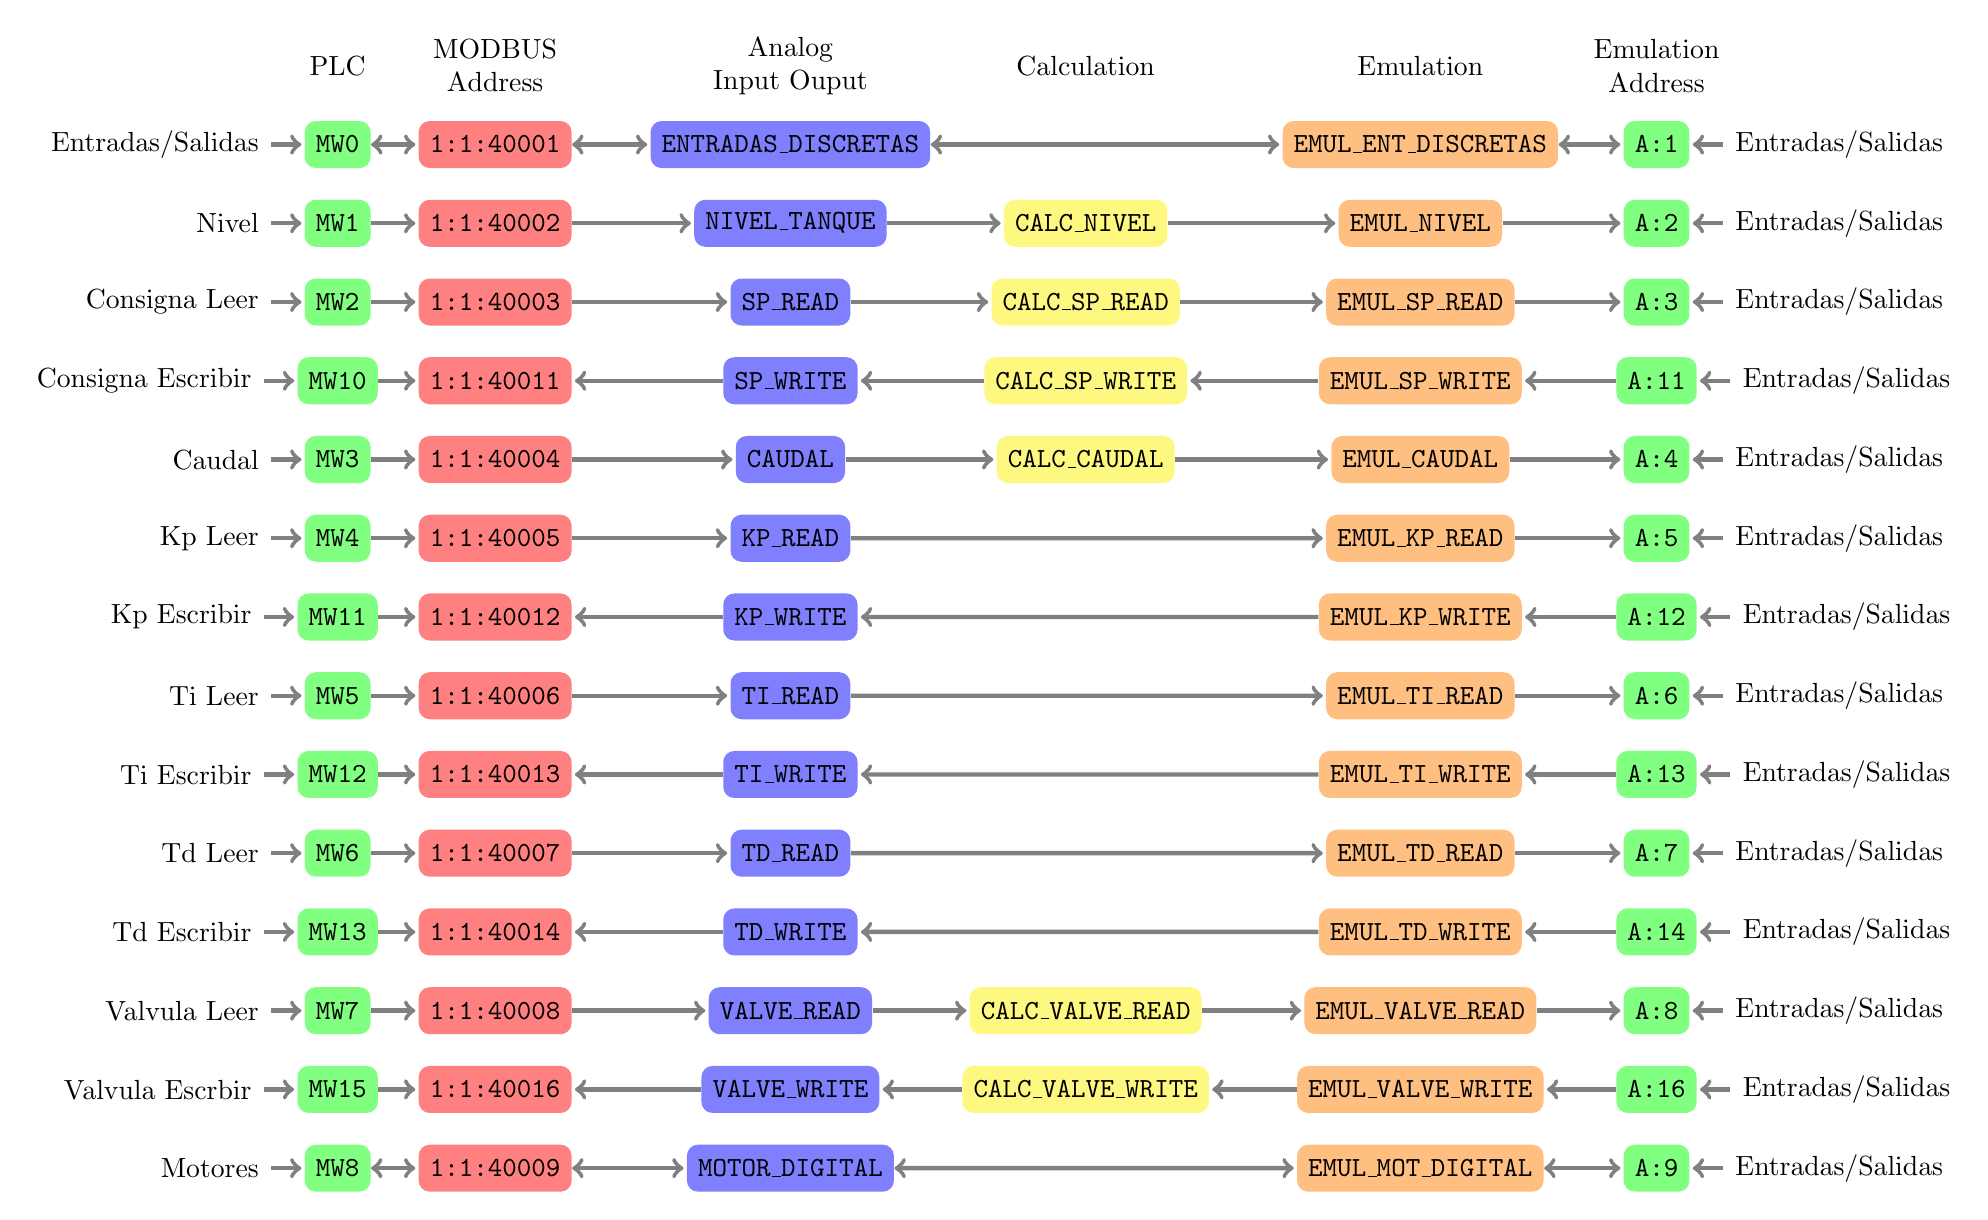
\begin{tikzpicture}[shorten >=1pt,->,draw=black!50]
    \tikzstyle{every pin edge}=[<-,shorten <=1pt, ultra thick]
    \tikzstyle{neuron}=[rectangle,fill=black!25,minimum size=17pt,inner 
sep=4pt, rounded corners]
    \tikzstyle{annot} = [text width=7em, text centered]

    \tikzstyle{plc neuron}=[neuron, fill=green!50];
    \tikzstyle{modbus neuron}=[neuron, fill=red!50, node 
    distance=0.4*5cm];
    \tikzstyle{aio neuron}=[neuron, fill=blue!50, node 
    distance=0.75*5cm];
    \tikzstyle{calc neuron}=[neuron, fill=yellow!50, node 
    distance=0.75*5cm];
    \tikzstyle{emul neuron}=[neuron, fill=orange!50, node 
    distance=0.85*5cm];
    \tikzstyle{emula neuron}=[neuron, fill=green!50, node 
    distance=0.6*5cm];

    % Draw the plc layer nodes
     \node[plc neuron, pin=left:Entradas/Salidas] (mw0) at (0,0) 
{\texttt{MW0}};
     \node[plc neuron, pin=left:Nivel] (mw1) at (0,-1) 
{\texttt{MW1}};
     \node[plc neuron, pin=left: Consigna Leer] (mw2) at (0,-2) 
{\texttt{MW2}};
     \node[plc neuron, pin=left: Consigna Escribir] (mw10) at (0,-3) 
{\texttt{MW10}};
     \node[plc neuron, pin=left: Caudal] (mw3) at (0,-4) 
{\texttt{MW3}};
      \node[plc neuron, pin=left: Kp Leer] (mw4) at (0,-5) 
 {\texttt{MW4}};
      \node[plc neuron, pin=left: Kp Escribir] (mw11) at (0,-6) 
 {\texttt{MW11}};
      \node[plc neuron, pin=left: Ti Leer] (mw5) at (0,-7) 
 {\texttt{MW5}};
      \node[plc neuron, pin=left: Ti Escribir] (mw12) at (0,-8) 
 {\texttt{MW12}};
      \node[plc neuron, pin=left: Td Leer] (mw6) at (0,-9) 
 {\texttt{MW6}};
      \node[plc neuron, pin=left: Td Escribir] (mw13) at (0,-10) 
 {\texttt{MW13}};
      \node[plc neuron, pin=left: Valvula Leer] (mw7) at (0,-11) 
 {\texttt{MW7}};
      \node[plc neuron, pin=left: Valvula Escrbir] (mw15) at (0,-12) 
 {\texttt{MW15}};
      \node[plc neuron, pin=left: Motores] (mw8) at (0,-13) 
 {\texttt{MW8}};

    %Draw Modbus layer nodes
    \node[modbus neuron, right of=mw0] (40001)  {\texttt{1:1:40001}};
    \node[modbus neuron, right of=mw1] (40002)  {\texttt{1:1:40002}};
    \node[modbus neuron, right of=mw2] (40003)  {\texttt{1:1:40003}};
    \node[modbus neuron, right of=mw3] (40004)  {\texttt{1:1:40004}};
    \node[modbus neuron, right of=mw4] (40005)  {\texttt{1:1:40005}};
    \node[modbus neuron, right of=mw5] (40006)  {\texttt{1:1:40006}};
    \node[modbus neuron, right of=mw6] (40007)  {\texttt{1:1:40007}};
    \node[modbus neuron, right of=mw7] (40008)  {\texttt{1:1:40008}};
    \node[modbus neuron, right of=mw8] (40009)  {\texttt{1:1:40009}};
    \node[modbus neuron, right of=mw10] (40011)  {\texttt{1:1:40011}};
    \node[modbus neuron, right of=mw11] (40012)  {\texttt{1:1:40012}};
    \node[modbus neuron, right of=mw12] (40013)  {\texttt{1:1:40013}};
    \node[modbus neuron, right of=mw13] (40014)  {\texttt{1:1:40014}};
    \node[modbus neuron, right of=mw15] (40016)  {\texttt{1:1:40016}};
     
    %Draw Analog Input Output layer nodes
    \node[aio neuron, right of=40001] (io)  {\texttt{ENTRADAS\_DISCRETAS}};
    \node[aio neuron, right of=40002] (niv)  {\texttt{NIVEL\_TANQUE}};
    \node[aio neuron, right of=40003] (spr)  {\texttt{SP\_READ}};
    \node[aio neuron, right of=40004] (caudal)  {\texttt{CAUDAL}};
    \node[aio neuron, right of=40005] (kpr)  {\texttt{KP\_READ}};
    \node[aio neuron, right of=40006] (tir)  {\texttt{TI\_READ}};
    \node[aio neuron, right of=40007] (tdr)  {\texttt{TD\_READ}};
    \node[aio neuron, right of=40008] (vr)  {\texttt{VALVE\_READ}};
    \node[aio neuron, right of=40009] (md)  {\texttt{MOTOR\_DIGITAL}};
    \node[aio neuron, right of=40011] (spw)  {\texttt{SP\_WRITE}};
    \node[aio neuron, right of=40012] (kpw)  {\texttt{KP\_WRITE}};
    \node[aio neuron, right of=40013] (tiw)  {\texttt{TI\_WRITE}};
    \node[aio neuron, right of=40014] (tdw) {\texttt{TD\_WRITE}};
    \node[aio neuron, right of=40016] (vw)  {\texttt{VALVE\_WRITE}};

    %Draw Calculation
    \node[calc neuron, right of=niv] (cniv) {\texttt{CALC\_NIVEL}};
    \node[calc neuron, right of=spr] (cspr) {\texttt{CALC\_SP\_READ}};
    \node[calc neuron, right of=spw] (cspw) {\texttt{CALC\_SP\_WRITE}};
    \node[calc neuron, right of=caudal] (ccaudal) {\texttt{CALC\_CAUDAL}};
    \node[calc neuron, right of=vr] (cvr) {\texttt{CALC\_VALVE\_READ}};
    \node[calc neuron, right of=vw] (cvw) {\texttt{CALC\_VALVE\_WRITE}};
    
    %Draw ResultCalculation
    \node[emul neuron, right of=cniv] (eniv) {\texttt{EMUL\_NIVEL}};
    \node[emul neuron, right of=cspr] (espr) {\texttt{EMUL\_SP\_READ}};
    \node[emul neuron, right of=cspw] (espw) {\texttt{EMUL\_SP\_WRITE}};
    \node[emul neuron, right of=ccaudal] (ecaudal) {\texttt{EMUL\_CAUDAL}};
    \node[emul neuron, right of=cvr] (evr) {\texttt{EMUL\_VALVE\_READ}};
    \node[emul neuron, right of=cvw] (evw) {\texttt{EMUL\_VALVE\_WRITE}};
    
    %Draw Emulation
    \node[emul neuron] (eio) at (2.75*5cm,0 cm) 
{\texttt{EMUL\_ENT\_DISCRETAS}};
    \node[emul neuron] (ekpr) at (2.75*5cm,-5 cm) 
{\texttt{EMUL\_KP\_READ}};
    \node[emul neuron] (etir) at (2.75*5cm,-7 cm) 
{\texttt{EMUL\_TI\_READ}};
    \node[emul neuron] (etdr) at (2.75*5cm,-9 cm) 
{\texttt{EMUL\_TD\_READ}};
    \node[emul neuron] (emd) at (2.75*5cm,-13 cm) 
{\texttt{EMUL\_MOT\_DIGITAL}};
    \node[emul neuron] (ekpw) at (2.75*5cm,-6 
cm){\texttt{EMUL\_KP\_WRITE}};
    \node[emul neuron] (etiw) at (2.75*5cm,-8 cm) 
{\texttt{EMUL\_TI\_WRITE}};
    \node[emul neuron] (etdw) at (2.75*5cm,-10 cm) 
{\texttt{EMUL\_TD\_WRITE}};

    %Draw internal variables
   \node[emula neuron, pin=right:Entradas/Salidas,right of=eio] (a1) 
  {\texttt{A:1}};
  \node[emula neuron, pin=right:Entradas/Salidas,right of=eniv] (a2) 
  {\texttt{A:2}};
  \node[emula neuron, pin=right:Entradas/Salidas,right of=espr] (a3) 
  {\texttt{A:3}};
  \node[emula neuron, pin=right:Entradas/Salidas,right of=espw] (a11) 
  {\texttt{A:11}};
  \node[emula neuron, pin=right:Entradas/Salidas,right of=ecaudal] (a4) 
  {\texttt{A:4}};
  \node[emula neuron, pin=right:Entradas/Salidas,right of=ekpr] (a5) 
  {\texttt{A:5}};
  \node[emula neuron, pin=right:Entradas/Salidas,right of=ekpw] (a12) 
  {\texttt{A:12}};
  \node[emula neuron, pin=right:Entradas/Salidas,right of=etir] (a6) 
  {\texttt{A:6}};
  \node[emula neuron, pin=right:Entradas/Salidas,right of=etiw] (a13) 
  {\texttt{A:13}};
  \node[emula neuron, pin=right:Entradas/Salidas,right of=etdr] (a7) 
  {\texttt{A:7}};
  \node[emula neuron, pin=right:Entradas/Salidas,right of=etdw] (a14) 
  {\texttt{A:14}};
  \node[emula neuron, pin=right:Entradas/Salidas,right of=evr] (a8) 
  {\texttt{A:8}};
  \node[emula neuron, pin=right:Entradas/Salidas,right of=evw] (a16) 
  {\texttt{A:16}};
  \node[emula neuron, pin=right:Entradas/Salidas,right of=emd] (a9) 
  {\texttt{A:9}};

   
  % Connect every node 
  %PLC -> MODBUS
  \path (mw0) edge[<->,ultra thick] (40001); 
  \path (mw1) edge[ultra thick] (40002); 
  \path (mw2) edge[ultra thick] (40003);
  \path (mw3) edge[ultra thick] (40004); 
  \path (mw4) edge[ultra thick] (40005); 
  \path (mw5) edge[ultra thick] (40006); 
  \path (mw6) edge[ultra thick] (40007); 
  \path (mw7) edge[ultra thick] (40008); 
  \path (mw8) edge[<->,ultra thick] (40009);
  \path (mw10) edge[ultra thick] (40011); 
  \path (mw11) edge[ultra thick] (40012); 
  \path (mw12) edge[ultra thick] (40013);
  \path (mw13) edge[ultra thick] (40014); 
  \path (mw15) edge[ultra thick] (40016); 

  %MODBUS -> Analog IO
  \path (40001) edge[<->,ultra thick] (io); 
  \path (40002) edge[ultra thick] (niv); 
  \path (40003) edge[ultra thick] (spr);
  \path (40004) edge[ultra thick] (caudal);
  \path (40005) edge[ultra thick] (kpr);
  \path (40006) edge[ultra thick] (tir);
  \path (40007) edge[ultra thick] (tdr); 
  \path (40008) edge[ultra thick] (vr);
  \path (40009) edge[<->,ultra thick] (md); 
  \path (spw) edge[ultra thick] (40011); 
  \path (kpw) edge[ultra thick] (40012);
  \path (tiw) edge[ultra thick] (40013); 
  \path (tdw) edge[ultra thick] (40014);
  \path (vw) edge[ultra thick] (40016); 

  %Analog -> Calc
  \path (niv) edge[ultra thick] (cniv);
  \path (spr) edge[ultra thick] (cspr);
  \path (cspw) edge[ultra thick] (spw);
  \path (caudal) edge[ultra thick] (ccaudal);
  \path (vr) edge[ultra thick] (cvr);
  \path (cvw) edge[ultra thick] (vw);

  %Calc -> Emulation
  \path (cniv) edge[ultra thick] (eniv);
  \path (cspr) edge[ultra thick] (espr);
  \path (espw) edge[ultra thick] (cspw);
  \path (ccaudal) edge[ultra thick] (ecaudal);
  \path (cvr) edge[ultra thick] (evr);
  \path (evw) edge[ultra thick] (cvw); 
  
  %Analog IO -> Emulation
  \path (io) edge[<->,ultra thick] (eio);
  \path (kpr) edge[ultra thick] (ekpr);
  \path (ekpw) edge[ultra thick] (kpw);
  \path (tir) edge[ultra thick] (etir);
  \path (etiw) edge[ultra thick] (tiw);
  \path (tdr) edge[ultra thick] (etdr);
  \path (etdw) edge[ultra thick] (tdw);
  \path (md) edge[<->,ultra thick] (emd);

  %Emulation -> Address
  \path (eio) edge[<->,ultra thick] (a1);
  \path (eniv) edge[ultra thick] (a2);
  \path (espr) edge[ultra thick] (a3);
  \path  (a11) edge[ultra thick] (espw);
  \path (ecaudal) edge[ultra thick] (a4);
  \path (ekpr) edge[ultra thick] (a5);
  \path  (a12) edge[ultra thick] (ekpw);
  \path (etir) edge[ultra thick] (a6);
  \path  (a13) edge[ultra thick] (etiw);
  \path (etdr) edge[ultra thick] (a7);
  \path (a14) edge[ultra thick] (etdw);
  \path (evr) edge[ultra thick] (a8);
  \path (a16) edge[ultra thick] (evw);
  \path (emd) edge[<->,ultra thick] (a9);
  

 
  % Annotate the layers
  \node[annot,above of=mw0, node distance=1cm] (plc) {PLC};
  \node[annot,above of=40001, node distance=1cm] (modbus) {MODBUS Address};
  \node[annot,above of=io, node distance=1cm] (aio) {Analog Input Ouput};
  \node[annot,right of=aio, node distance=0.75*5cm] (calc) {Calculation};
  \node[annot,above of=eio, node distance=1cm] (emul) {Emulation};
  \node[annot,above of=a1, node distance=1cm] (emula) {Emulation Address};

\end{tikzpicture}
  }
    \caption{Conexion de bloques de la Base de Datos}
    \label{fig:bloqDB}
\end{figure*}

La configuracion de los bloques debe ser tal que para:
\begin{itemize}
  \item Analog Input/Output: Address debe tener el valor de MODBUS Address 
  correspondiente. El Target esta dado por la punta de la flecha que se origina 
  en ese bloque.
  \item Calculation: Parameter es el bloque entretante y Target es el bloque 
  saliente en el esquema.
  \item Analog Emulation: Address toma el valor de Emulation Address y el 
  Target es el bloque al que apunta la flecha. 
\end{itemize}



\subsubsection{Creación de los bloques de la base de datos}
A continuación se muestran los pasos necesarios para la creación de un elemento 
de la base de datos (Ver Tab.\ref{tab:confBlockDB}).
% \begin{enumerate}
%  \item Active P-CIM para Windows utilizando el Startup de P-CIM.
%  \item En el directorio de P-CIM oprima el icono del Editor de la Base de Datos.
%  \item Oprima la tecla Add. El Editor de la Base de Datos despliega la ventana de
%   especificaciones de Valor Analógico.
%  \item Ingrese el nombre y complete los campos que correspondan en cada 
% bloque. No se han utilizado
%  el resto de las opciones que presenta la base de datos excepto aquellos que fueron expresados anteriormente 
%  en la tabla \todo{agregar tabla}
%  \item Oprima la tecla OK para regresar al directorio del Bloque.
%  \item Oprima la tecla Save DB para guardar la Base de Datos.
% \end{enumerate}
\begin{table}[!ht]
\centering
\renewcommand*{\arraystretch}{0.01}
\begin{tabular}{*{2}{m{0.45\textwidth}}}
\hline
  Active P-CIM utilizando el Startup de P-CIM. En el sub-directorio Development 
  de P-CIM oprima el icono del Editor de la Base de Datos
  &\begin{center}
    %\rule{0.4\textwidth}{0.3\textwidth}
    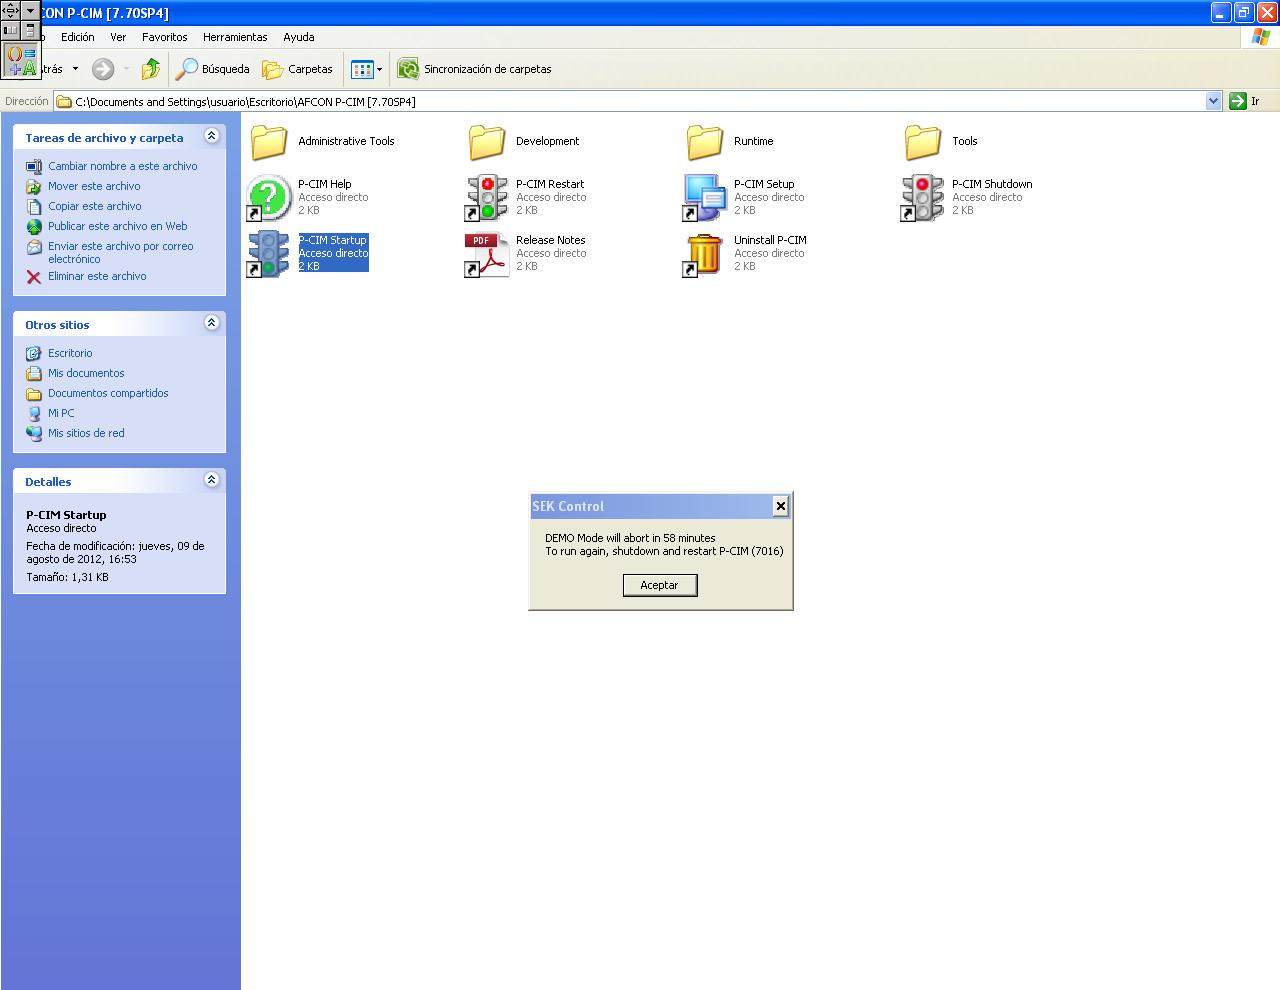
\includegraphics[width=0.4\textwidth]
      {Cap5-SCADA/images/startUp.jpeg}
  \end{center}\\
\hline
    Dentro del Editor de la Base de Datos se desplegara la ventana de Block 
    Directory. En esta ultima se muestran los bloques que han sido creados y 
    están clasificados en las pestañas según su tipo.  Oprima la tecla Add, se 
    despliega la ventana de especificaciones de Valor Analógico 
    &\begin{center}
      %\rule{0.4\textwidth}{0.3\textwidth}
      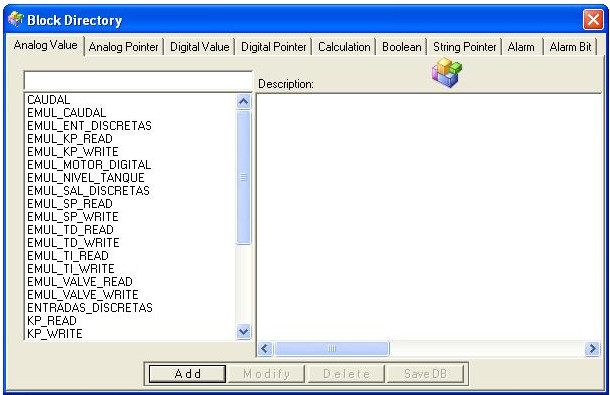
\includegraphics[width=0.4\textwidth]
	{Cap5-SCADA/images/database.jpeg}
    \end{center}\\
\hline
    Ingrese el nombre y complete los campos que correspondan en cada bloque. 
    No se han utilizado el resto de las opciones que presenta la base de datos 
    excepto aquellos que fueron expresados anteriormente 
    Oprima la tecla OK para regresar al directorio del Bloque.
    y Save DB para guardar la Base de Datos.
    &\begin{center}
      %\rule{0.4\textwidth}{0.3\textwidth}
      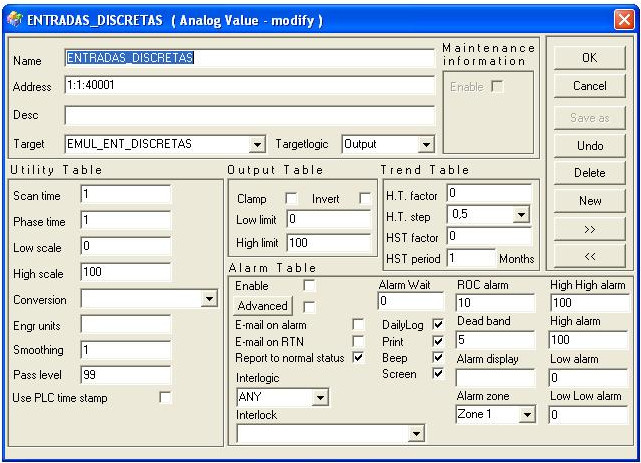
\includegraphics[width=0.4\textwidth]
	{Cap5-SCADA/images/database1.jpeg}
    \end{center}\\
\hline
\end{tabular}
\caption{Configuración de los bloques de la base de datos.}
\label{tab:confBlockDB}
\end{table}



Ahora podemos controlar el funcionamiento del bloque recién configurado de la 
siguiente manera:
\begin{enumerate}
  \item Abra el Datascope (Monitor de Datos), con un doble click sobre su icono 
  en el directorio de P-CIM.
  \item Escriba el nombre de alguno de los bloques antes definidos  y en otro 
  item su dirección.
  \item Se debe poder observar en ambos el mismo valor leído(en caso de 
  registros de lectura) o el mismo valor al escribir en uno u otro de los items.
\end{enumerate}
Si esta prueba nos ha dado los resultados esperados podemos estar seguros que 
nuestros bloques se encuentran bien configurados y podemos proseguir con el 
desarrollo de nuestro sistema \gls{scada}.


\subsection{Capa de aplicación}
\label{subsec:CapaAplicacion}
La tercer y última capa del sistema \gls{scada} es la capa de aplicación. Esta 
será utilizada en nuestro \gls{pfe} unicamente como \gls{hmi}. Para el 
desarrollo de la interfaz gráfica definimos un documento gráfico creado con el 
Editor de Animaciones (Animation Editor). Finalmente, mediante el Servidor de 
Pantallas (Operator Workstation) se pone en marcha el sistema. A continuación se 
presentan el desarrollo y descripción de la pantalla realizada mediante las 
herramientas gráficas provistas por P-CIM.

%Incluye ilustraciones, indicadores y controles emulando un panel de control 
%real pero con muchos más elementos. Actúa como interfase entre el operador y 
%la planta.


\subsubsection{Diseño de una pantalla}
El primer paso en el diseño de un pantalla es la definición de requerimientos 
con los que debemos cumplir. Estos se resumen en:
\begin{itemize}
 \item Botones de encendido y parada de la planta.
 \item Visualización del estado actual de la planta: Niveles, caudal, bombas 
 encendidas, etc.
 \item Control Manual
 \begin{itemize}
  \item Encender las bombas de manera independiente.
  \item Controlar la abertura de la válvula
 \end{itemize}
 \item Control Automático
 \begin{itemize}
  \item Visualizar el seguimiento de la consigna.
  \item Visualizar/Definir la consigna
  \item Visualizar/Definir las constantes del controlador
 \end{itemize}
\end{itemize}

Ahora mediante el Editor de Animaciones (ubicado en el sub-directorio 
Development) diseñamos y definimos las características funcionales de 
la pantalla que correrá en el Operator Workstation. 


Para la realización de dicha interfaz se procedió en el siguiente orden:(Ver 
Tab.\ref{tab:diseñoAnimGraf})
% \begin{enumerate}
%  \item Iniciar el Editor de Animaciones. Elegir el icono de la carpeta de 
%   P-CIM. Aparece un pantalla sin nombre. Guarde el archivo asignándole un 
%   nombre.
%  \item Crear la ilustración básica.\\
%     Use el Editor de Animaciones para  dibujar sus propios gráficos o insertar 
%     objetos gráficos ya creados de la biblioteca de ClipArt. Los objetos 
%     gráficos insertados desde el ClipArt pueden tratarse como cualquier otro 
%     objeto gráfico y ser movidos, redimensionados, editados y asignados con 
%     propiedades.
%     Para seleccionar un objeto de ClipArt:(Ver \todo{agregar tabla})
%     \begin{enumerate}
%       \item Elegir "’ClipArt” en el menú File, luego elegir la categoría en el submenú o elegir el botón 
%       categoría de la caja de ClipArt.
%       \item Hacer click en el objeto para seleccionarlo.
%       \item Hacer click nuevamente sobre el objeto seleccionado, mantener presionada la tecla CTRL y 
%       el botón izquierdo del mouse, arrastrar el objeto hasta el lugar deseado en el pantalla y soltar 
%       el botón del mouse y la tecla CTRL. La ventana de ClipArt se cierra tan pronto Ud. comienza a 
%       arrastrar el objeto.
%     \end{enumerate}
%     
%  \item Animar la ilustración.\\
%       Para animar un objeto gráfico se debe seleccionar el objeto y especificar una o
%       más propiedades de la Lista de Propiedades (Properties List).
%       Para comenzar a animar un objeto
%       \begin{enumerate}
% 	\item Seleccionar el objeto (click izquierdo del mouse); por ejemplo un rectángulo. El
% 	Editor de Animaciones le coloca marcas al objeto.
% 	\item Elegir Properties List (Lista de Propiedades) 
%       \end{enumerate}
%       Las propiedades están divididas en tres
%       categorías principales: Controls, Indicators y Special 
%       (controles, indicadores y especiales).
%       \begin{itemize}
% 	\item  Controls: especifica una entrada de datos la cual puede estar dada por 
% 	casillas de entrada de datos, botones que inician acciones, o
% 	potenciómetros que permiten fijar valores analógicos.
% 	\item Indicators: Usados para crear presentaciones textuales, de color
% 	y gráficas de los datos, en estos los contenidos, posición, color y
% 	tamaño cambian en función del valor de los datos.
% 	\item Special: esta categoría es usada para especificar Gráficos de Tendencia o
% 	“Medidores de Desviación”.
%       \end{itemize}
%       Un signo de visto en una casilla de propiedades significa que ésta es la propiedad
%       asignada al objeto gráfico. Luego aparece otra ventana de diálogo:
%       donde se debe completar (Servidor, Tópico e Item) para cada
%       propiedad que especifique (excepto para el botón). Esto designa
%       respectivamente el origen de los datos mostrados por el indicador o 
%       el destino de los datos escritos por el objeto de control.
%       
%  \item Probar los resultados en el Operator Workstation.\\
%       Para poder probar el funcionamiento de nuestra \gls{hmi} procedemos de la siguiente manera:
%       \begin{enumerate}
%        \item 
%       \end{enumerate}
% \end{enumerate}
\begin{table}[H]
\centering
\renewcommand*{\arraystretch}{0.01}
\begin{tabular}{*{2}{m{0.435\textwidth}}}
   \hline
	Iniciar el Editor de Animaciones que se encuentra en el sub-directorio 
	Development. Aparece un pantalla sin nombre "untitled". Guarde el 
archivo 	asignándole un nombre.
	&\begin{center}
	  %\rule{0.4\textwidth}{0.3\textwidth}
	 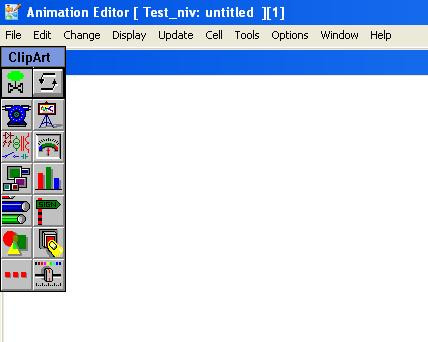
\includegraphics[width=0.4\textwidth]
	{Cap5-SCADA/images/animEdit.jpeg}
	\end{center}\\
   \hline
	Crear la ilustración básica con el Editor de Animaciones para  
	dibujar sus propios gráficos o insertar objetos gráficos de 
	la biblioteca de ClipArt. Los objetos gráficos insertados pueden ser 
	movidos, redimensionados, editados y asignarle propiedades.
	&\begin{center}
	  %\rule{0.4\textwidth}{0.3\textwidth}
	   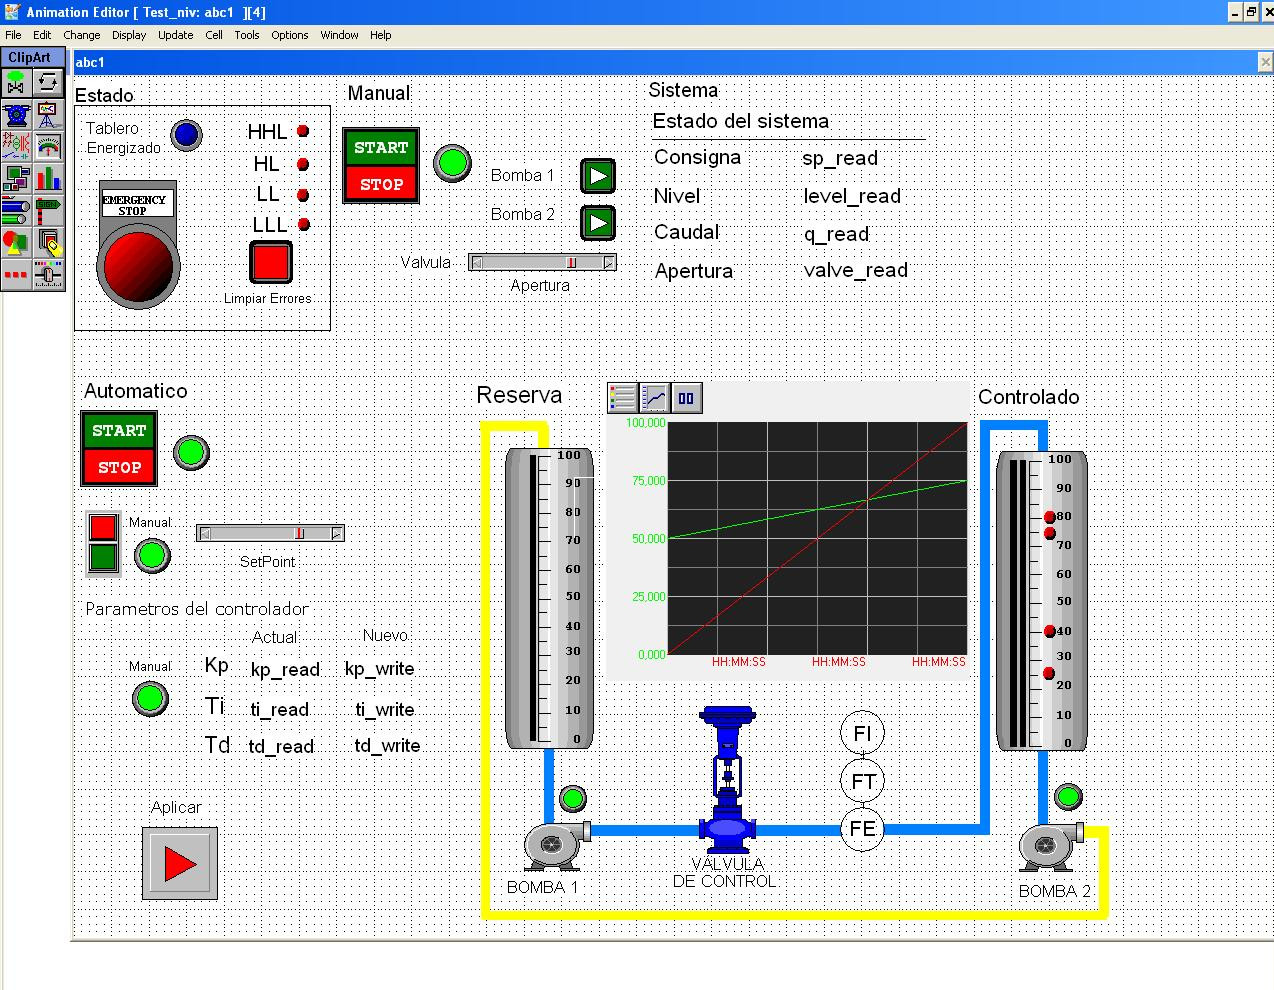
\includegraphics[width=0.4\textwidth]
	{Cap5-SCADA/images/animEdit1.jpeg}
	\end{center}\\
   \hline
	  Para animar un objeto gráfico se debe seleccionar 
	  el objeto (click izquierdo del mouse). El Editor de Animaciones le 
	  coloca marcas al objeto. Elegir Properties List (Lista de 
	  Propiedades). Un signo de visto en una casilla de propiedades 
	  significa que ésta es la propiedad asignada al objeto gráfico. 
	&\begin{center}
	  %\rule{0.4\textwidth}{0.3\textwidth}
	   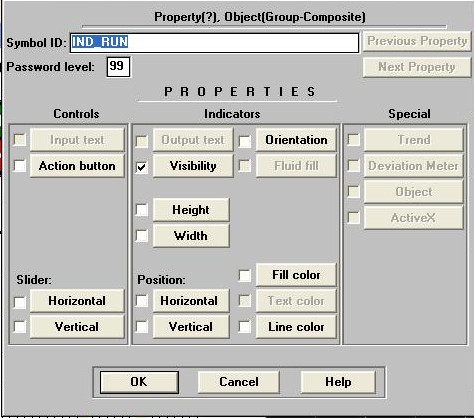
\includegraphics[width=0.4\textwidth]
	{Cap5-SCADA/images/animEdit2.jpeg}
	\end{center}\\
   \hline
	  Luego aparece otra ventana de diálogo:
	  donde se debe completar (Servidor, Tópico e Item. Ver Sec. 
	  \ref{subsubsec:InforDriver}) para cada
	  propiedad que especifique. Esto designa
	  respectivamente el origen de los datos mostrados por el indicador o 
	  el destino de los datos escritos por el objeto de control. 
	&\begin{center}
	  %\rule{0.4\textwidth}{0.3\textwidth}
	   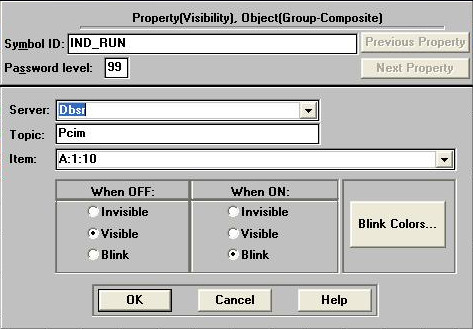
\includegraphics[width=0.4\textwidth]
	{Cap5-SCADA/images/animEdit3.jpeg}
	\end{center}\\
   \hline
      \end{tabular}
\caption{Diseño y animación de la interfaz gráfica.}
\label{tab:diseñoAnimGraf}
\end{table}


Las propiedades que pueden ser asignadas a un elemento gráfico están divididas 
en tres categorías principales: Controls, Indicators y Special (controles, 
indicadores y especiales). Como se puede ver \todo{agregar imagen}
\begin{itemize}
\item  Controls: especifica una entrada de datos la cual puede estar dada por 
	casillas de entrada de datos, botones que inician acciones, o
	potenciómetros que permiten fijar valores analógicos.
	
	
  \begin{figure}[!ht]
	\centering
	\begin{subfigure}[b]{0.2\textwidth}
	    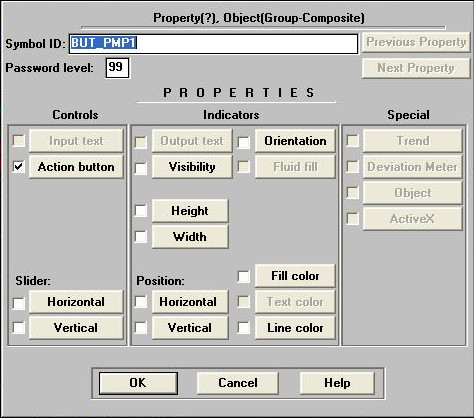
\includegraphics[width=\textwidth]{Cap5-SCADA/images/actbtn.jpeg}
	    \caption{}
	    \label{}
  	\end{subfigure}
	\begin{subfigure}[b]{0.2\textwidth}
	    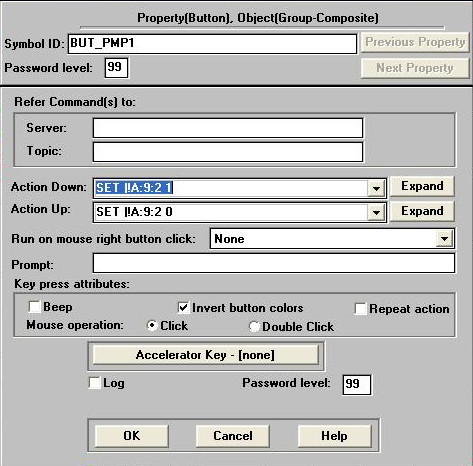
\includegraphics[width=\textwidth]{Cap5-SCADA/images/actbtn1.jpeg}
	    \caption{}
	    \label{}
  	\end{subfigure}
% 	\begin{subfigure}[3]{0.3\textwidth}
% 	    \includegraphics[width=\textwidth]{Cap5-SCADA/images/actbtn2.jpeg}}
% 	    \caption{}
% 	    \label{}
%   	\end{subfigure}
	\caption{Interfaz Gráfica del SCADA}
	\label{fig:controlshmi}
  \end{figure}
	
	
\item Indicators: usados para crear presentaciones textuales, de color
	y gráficas de los datos, en estos los contenidos, posición, color y
	tamaño cambian en función del valor de los datos.
  \begin{figure}[!ht]
	\centering
	\begin{subfigure}[b]{0.2\textwidth}
	   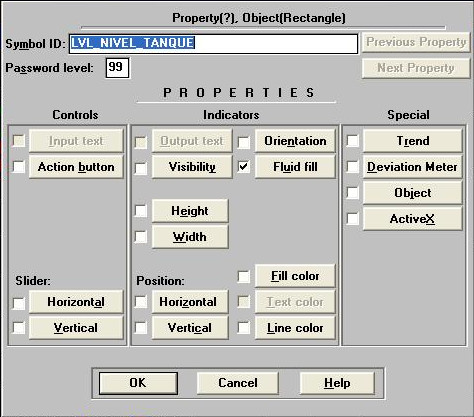
\includegraphics[width=\textwidth]{Cap5-SCADA/images/indicator.jpeg}
	    \caption{}
	    \label{}
  	\end{subfigure}
	\begin{subfigure}[b]{0.2\textwidth}
	   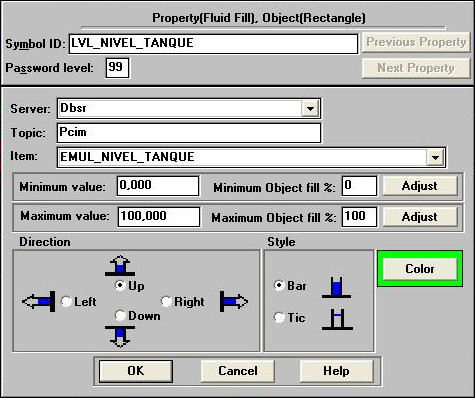
\includegraphics[width=\textwidth]{Cap5-SCADA/images/indicator1.jpeg}
	    \caption{}
	    \label{}
  	\end{subfigure}
% 	\begin{subfigure}[3]{0.3\textwidth}
% 	    \includegraphics[width=\textwidth]{Cap5-SCADA/images/actbtn2.jpeg}}
% 	    \caption{}
% 	    \label{}
%   	\end{subfigure}
	\caption{Interfaz Gráfica del SCADA}
	\label{fig:indicatorhmi}
  \end{figure}
	
\item Special: esta categoría es usada para especificar Gráficos de Tendencia o
	“Medidores de Desviación”.
\end{itemize}
  \begin{figure}[!ht]
	\centering
	\begin{subfigure}[b]{0.2\textwidth}
	   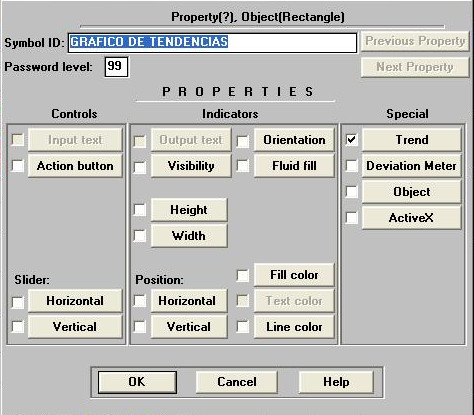
\includegraphics[width=\textwidth]{Cap5-SCADA/images/tendencia.jpeg}
	    \caption{}
	    \label{}
  	\end{subfigure}
	\begin{subfigure}[b]{0.2\textwidth}
	   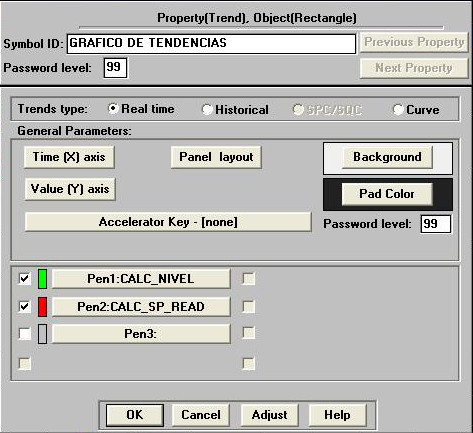
\includegraphics[width=\textwidth]{Cap5-SCADA/images/tendencia1.jpeg}
	    \caption{}
	    \label{}
  	\end{subfigure}
	\begin{subfigure}[b]{0.2\textwidth}
	   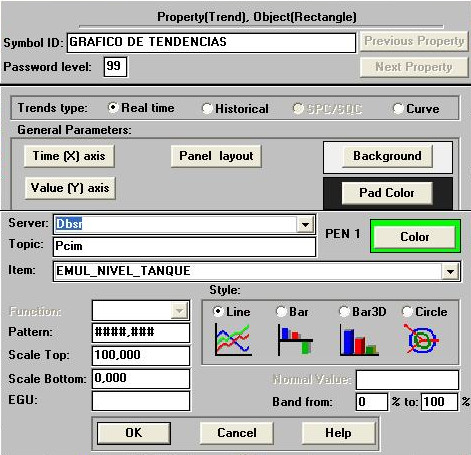
\includegraphics[width=\textwidth]{Cap5-SCADA/images/tendencia2.jpeg}
	    \caption{}
	    \label{}
  	\end{subfigure}
	\begin{subfigure}[b]{0.2\textwidth}
	   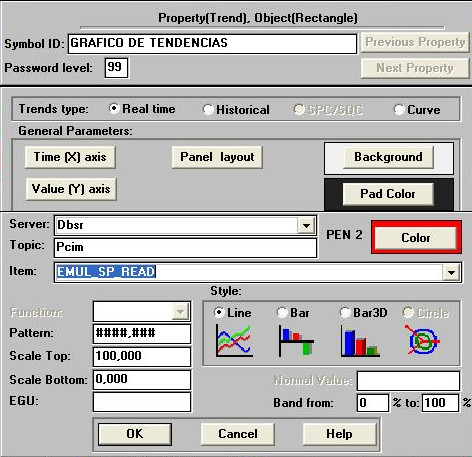
\includegraphics[width=\textwidth]{Cap5-SCADA/images/tendencia3.jpeg}
	    \caption{}
	    \label{}
  	\end{subfigure}
	\caption{Interfaz Gráfica del SCADA}
	\label{fig:tendhmi}
  \end{figure}


Mediante las características antes especificadas se obtuvo el resultado que se 
observa en la figura \ref{fig:hmiscada}.
  \begin{figure}[!ht]
	\centering
	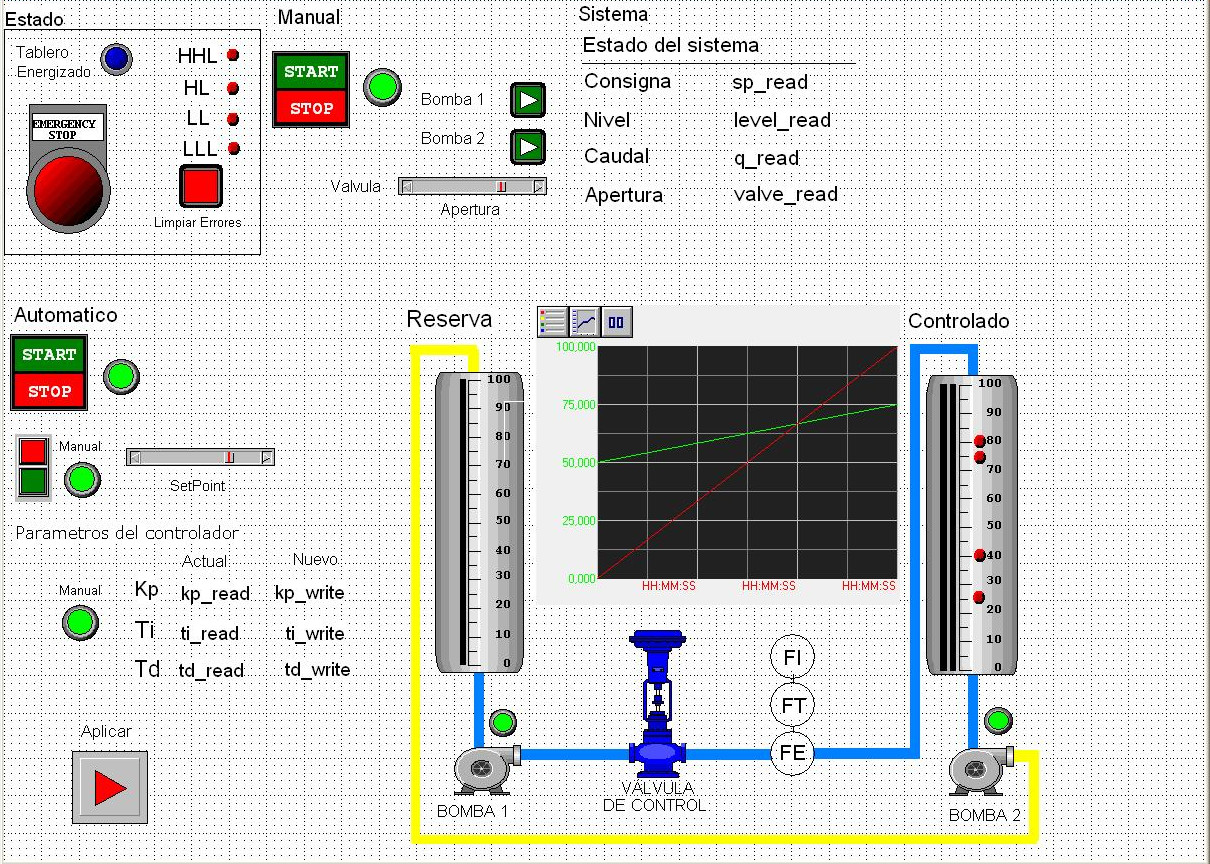
\includegraphics[width=0.8\textwidth]
	{Cap5-SCADA/images/hmiScada.jpeg}
	\caption{Interfaz Gráfica del SCADA}
	\label{fig:hmiscada}
  \end{figure}

\section{Ejecución}
\label{sec:Ejecucion}
Una ves que han sido configuradas cada una de las partes podemos utilizar 
nuestro sistema SCADA. Para poder probar el funcionamiento de nuestra \gls{hmi} 
procedemos de la manera que se describe en la Tab.\todo{agregar tabla }